\chapter{Introduzione all'analisi numerica nell'integrazione}

Il problema dell'integrazione numerica può essere risolto, in linea di principio, con l'aiuto di equazioni differenziali ordinarie (\underline{ODEs}):
\[ \int^x_a\, f(y)\, dy\ =\ g(x) \quad \quad \Rightarrow \quad \quad \frac{d\, g}{d\, x}\ =\ f(x)\ , \]
con boundary $x_0=a$.

Sebbene questa osservazione sia formalmente corretta, è preferibile sviluppare metodi diretti di integrazione numerica, analogamente a quanto si è fatto per le equazioni differenziali, dove la scelta del metodo appropriato non è affatto immediata.

Un algoritmo generale di integrazione numerica ha la struttura

\[
\int_a^b f(x)\,dx = \sum_i w_i f(x_i),
\]

dove $w_i$ sono pesi e $x_i$ i nodi di valutazione. 

In genere si pone $x_i = a + i h$ con passo $h$ uniforme e si scrive $f_i = f(x_i)$.

\begin{multicols}{2}	
	Si distinguono due grandi classi di formule:
	
	\begin{itemize}
		\item \textbf{Formule chiuse}: utilizzano anche i valori agli estremi $a$ e $b$.
		\item \textbf{Formule aperte}: non utilizzano uno o entrambi gli estremi.
	\end{itemize}
	
	Il vantaggio principale delle formule aperte è che possono essere utilizzate quando la funzione non è definita agli estremi, pur essendo l'integrale ben definito.
	
	\begin{figure}[H]
		\centering
		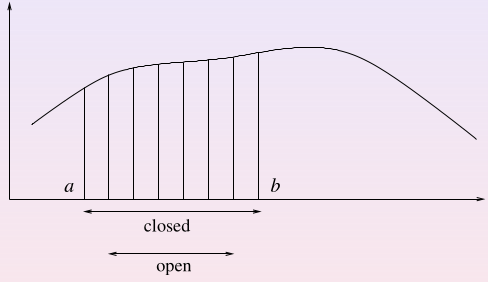
\includegraphics[width=\linewidth]{img/integration_1.png}
		\caption{differenza fra intervalli presi in considerazione da classi di formule chiuse e aperte}
	\end{figure}
\end{multicols}



\subsection{Formule di Newton–Cotes su intervallo singolo}

Le formule di Newton-Cotes nascono dalla divisione in intervalli equispaziati e dalla successiva integrazione esatta di un polinomio che passa per quegli $n$ punti (interpolazione).

La regola fondamentale dell'integrazione numerica, la formula di Newton-Cotes di grado più basso è la \underline{regola dei trapezi}, che usa una retta tesa fra due punti successivi per interpolare:

\begin{equation}
	\label{trapezoidal-rule}
	\int_{x_1}^{x_2}\, f(x)\, dx\ =\
	\frac{1}{2}\, h \, [f_1 + f_2] + \mathcal{O}(h^3\, f^{''})\ ,\
\end{equation}  

questa è esatta per funzioni lineari, ad esempio $f(x)=x$. 

Si ottiene interpolando $f(x)$ con il polinomio lineare che passa per i punti $(x_1,\, f_1)$ e $(x_2,\, f_2)$:

\[ f(x)\ =\ f_1\, +\, (f_2\, -\, f_1)\, x\ \ , \]

e in seguito integrando sull'intervallo normalizzato $0 \le x \le 1$.

Formule di ordine superiore si ottengono interpolando con polinomi di grado più elevato. Ad esempio,

\begin{equation}\label{Simpson's rule}
	\int_{x_1}^{x_3}\, f(x)\, dx\ =\ h\, \left[
	\frac{1}{3}\, f_1\, +\, \frac{4}{3}\, f_2\, +\, \frac{1}{3}\, f_3\right]\, +\,	\mathcal{O}(h^5\, f^{(4)})\ \ ,
\end{equation} 

che è la \underline{regola di Simpson}, esatta per polinomi fino al terzo grado.
La regola di Simpson nasce dall'interpolazione con una parabola $P(x)=Ax^x + Bx+C$ su tre punti equispaziati $x_0$, $x_1$, $x_2$ con funzione da integrare $f_0=f(x_0)$, $f_1$, $f_2$. Facciamo un cambio di variabile $t=x-x_i$ così che i tre punti diventino $t=0,\, h,\, 2h$, riscrivendo la parabola come $P(t)=at^2+bt+c$. Si va ora ad imporre che $P(t=0)=c=f_0$, mentre nel secondo punto $P(t=h)=ah^2+b^h+c=f_1$ e nel terzo $P(t=2h)=4ah^2+2bh+c=f_2$. Invertendo questo sistema di equazioni si trova che $c=f_0$, $a=\frac{f_2-2f_1+f_0}{2h^2}$ mentre $b=\frac{f_1-f_0}{h}-ah$.
A questo punto l'integrale $\int_{x_0}^{x_2} f(x) dx\approx \int_0^{2h} P(t) dt= \int_0^{2h} at^2+bt+f_0 dt$ è facilmente sostituibile con le dovute sostituzioni di $a$ e $b$ nelle forme appena trovate e con una semplice integrazione del polinomio si ottiene proprio Simpson: $\int_{x_0}^{x_2} f(x) dx\approx \frac{h}{3} [f_0 + 4\,f_1 + f_2]$.

Analogamente, per cinque punti la formula di Newton-Cotes diventa:

\[ \int_{x_1}^{x_5}\, f(x)\, dx\ =\ h\, \left[ \frac{14}{45}\, f_1\, +\, \frac{64}{45}\, f_2\, +\, \frac{24}{45}\, f_3\, +\, \frac{64}{45}\, f_4\, +\, \frac{14}{45}\, f_5\, \right]\, +\, \mathcal{O}(h^7\, f^{(6)})\ \ .\]

\subsection{Alcune formule locali}

È utile osservare anche relazioni locali su intervalli elementari:

\[ \int_{x_0}^{x_1}\, f(x)\, dx\ =\ h[f_1]\, +\, \mathcal{O}(h^2\, f')\ \ ,\]


\[ \int_{x_0}^{x_1}\, f(x)\, dx\ =\ h\, \left[ \frac{3}{2}f_1\, -\, \frac{1}{2}f_2 \right]\, +\, \mathcal{O}(h^3\, f'')\ \ .\]

La prima è un semplice rettangolo, una Newton-Cotes aperta di ordine 0 con errore di ordine $h^2$, mentre la seconda formula è una Newton-Cotes aperta di ordine 1 e si ottiene interpolando linearmente $f(x)\ =\ f_1 + x\, (f_2 - f_1)$, e integrando nell'intervallo $-1 \le x \le 0$:

\[ \int_{-1}^{0} f(x)\,dx\ =\ -(-f_1)\, -\, \frac{(-1)^2}{2}\, (f_2 - f_1) \ =\ \left[ \frac{3}{2}f_1 - \frac{1}{2}f_2\right]\ .\]

Formule di ordine superiore si ottengono usando approssimazioni polinomiali di grado crescente.

\subsection{Intervalli estesi}

Passando a intervalli estesi, dalla regola dei trapezi in eq.(\ref{trapezoidal-rule}) segue una regola dei trapezi estesa:

\begin{equation} \label{regola-dei-trapezi-estesa}
	\int_{x_1}^{x_n} f(x)\,dx\ =\ h\, \left[
	\frac{1}{2}f_1\, +\, f_2\, +\, f_3\, +\, \dots\, +\, \frac{1}{2}f_n
	\right]\, +\,
	\mathcal{O}\!\left(\frac{(x_n-x_1)^3}{N^2}\, f''\right)\ \ ,
\end{equation} 

dove $N$ è il numero di suddivisioni.

Dalla regola di Simpson in eq.(\ref{Simpson's rule}), si ottiene invece:

\begin{equation}\label{Simpson-esteso}
	\int_{x_1}^{x_n}\, f(x)\,dx\ =\ h\, \left[ \frac{1}{3}f_1\,+\,\frac{4}{3}f_2\,+\,\frac{2}{3}f_3\,+\,\frac{4}{3}f_4\,\dots\,+\,\frac{4}{3}f_{n-1}\,+\,\frac{1}{3}f_n\right]
	\,+\,\mathcal{O}\!\left(\frac{1}{N^4}\right)\ \ .
\end{equation} 

Di seguito un'implementazione in C della regola dei trapezi e di Simpson:
\lstinputlisting[style=Cstyle,
	caption={Implementazione del metodo dei trapezi},
	label={lst:trapezi}]{trapezi.c}

Si può combinare una formula aperta locale (singolo intervallo) con una formula chiusa estesa di quelle appena scritte per ottenere una formula aperta su intervallo esteso. 

Ad esempio, combinando

\[
\int_{x_0}^{x_1} f(x)\,dx
=
h f_1 + \mathcal{O}(h^2 f')
\]

con la regola dei trapezi estesa su $[x_1,x_n]$ vista in eq.\ref{regola-dei-trapezi-estesa}, si ottiene:

\[ \int_{x_0}^{x_n}\, f(x)\, dx\ =\ h\, \left[ \frac{3}{2}f_1\, +\, f_2\, +\, f_3\, +\, \dots\, +\, \frac{3}{2}f_{n-1}\right]\,+\, \mathcal{O}\!\left(\frac{1}{N^2}\right)\ \ .\]

Analogamente, combinando la formula aperta di ordine superiore

\[ \int_{x_0}^{x_1} f(x)\,dx \ =\ h\,\left[ \frac{23}{12}f_1\,-\,\frac{16}{12}f_2\,+\,\frac{5}{12}f_3\right]\, +\, \mathcal{O}(h^4 f^{(3)})\ \ , \]

con la regola di Simpson estesa eq.(\ref{Simpson-esteso}), si ottiene una formula complessiva di ordine $\mathcal{O}(1/N^4)$.

\[ \int_{x_0}^{x_n}\, f(x)\, dx\ =\ h\, \left[ \frac{27}{12}f_1\, +\, 0\, +\, \frac{13}{12}f_3\, +\, \frac{4}{3} f_4\, +\,  \dots\, +\, \frac{4}{3}f_{n-4}, +\, \frac{13}{12}f_{n-3}\, +\, 0\, +\, \frac{27}{12}f_{n-1}\right]\,+\, \mathcal{O}\!\left(\frac{1}{N^2}\right)\ \ .\]

\bigskip

Il problema pratico fondamentale rimane: quanti passi bisogna utilizzare?

Se si usa la regola dei trapezi come blocco base, l'errore scala come $boxed{\frac{K}{N^2}}$, raddoppiando $N$, l'errore si riduce di un fattore 4. Questo comportamento è alla base dei metodi di raffinamento successivi.

\subsection{Valutazione dell’errore e formula esatta dei trapezi}

L'errore può essere valutato facendo la differenza fra l'integrale calcolato con N steps e quello calcolato con 2N steps.

Per stimare in modo più preciso l’errore della regola dei trapezi estesa, si può utilizzare la sua espressione esatta in termini dei numeri di Bernoulli:

\[
\int_{x_1}^{x_n} f(x)\,dx
\ =\
h\ \left[
\frac{1}{2}f_1\, +\, f_2\, +\, \dots\, +\, \frac{1}{2}f_n
\right]
\,-\,
\frac{B_2 h^2}{2!}\left(f'_n - f'_1\right)
\,-\,
\frac{B_{2k} h^{2k}}{(2k)!}\,
\left(f^{(2k-1)}_n\, -\, f^{(2k-1)}_1\right)
\,-\, \dots
\]

dove $B_k$ sono i numeri di Bernoulli, definiti tramite

\[
\frac{t}{e^t - 1}
\ =\
\sum_{n=0}^{\infty}\, B_n\, \frac{t^n}{n!}.
\]

Il termine dominante dell’errore è proporzionale a $h^2$, cioè a $1/N^2$. Se indichiamo con $S_N$ l’integrale calcolato con $N$ suddivisioni e con $S_{2N}$ quello con $2N$, possiamo eliminare il termine in $h^2$ combinando linearmente i due risultati:

\[
S = \frac{4}{3} S_{2N} - \frac{1}{3} S_N.
\]

In questo modo l’errore dominante diventa dell’ordine $h^4$.

\subsection{Integrazione di Romberg}

L’idea precedente può essere iterata. Se una combinazione elimina il termine in $h^2$, si può ripetere il procedimento per eliminare anche il termine in $h^4$, poi quello in $h^6$, e così via.

Il metodo di Romberg consiste nel:

\begin{itemize}
	\item calcolare l’integrale con una sequenza di suddivisioni $N, 2N, 4N, \dots$;
	\item costruire combinazioni lineari che eliminano progressivamente i termini dominanti dell’errore;
	\item interpretare il risultato come un’estrapolazione razionale nel limite $N \to \infty$.
\end{itemize}

Il metodo produce una tabella triangolare di approssimazioni con ordine crescente di accuratezza.

Di seguito un'implementazione in C dell'integrazione di Romberg presa dal \emph{Numerical Recipes in C: The art of scientific programming}:

\lstinputlisting[style=Cstyle,
				caption={Implementazione del metodo di Romberg},
				label={lst:romberg}]{Romberg.c}


\subsection{Quadrature Gaussiane}
Vogliamo approssimare integrali del tipo

\[\int W(x) f(x)\, dx\ =\ \sum_{j=1}^{N} w_j f(x_j)\ \ ,\]

dove: $W(x) > 0$ è una funzione peso, $\int W(x)\,dx = 1$ (normalizzazione) ed i nodi $x_j$ non sono necessariamente equispaziati.

Introduciamo il prodotto scalare pesato

\[\langle f\, |\, g \rangle\ =\ \int\, W(x)\, f(x)\, g(x)\, dx\ \ .\]

Si definisce una successione di polinomi ortogonali $\{p_k(x)\}$ tramite la ricorrenza a tre termini:

\[ p_{-1}(x)=0, \qquad p_0(x)=1\ \ ,\]

\[ p_{j+1}(x)\ =\ (x-a_j)\, p_j(x) - b_j\, p_{j-1}(x)\ \ ,\]

con coefficienti:

\[a_j = \frac{\langle x\, p_j\, |\, p_j \rangle}{\langle p_j\, |\, p_j \rangle},
\qquad
b_j =\frac{\langle p_j\, |\, p_j \rangle}{\langle p_{j-1}\, |\, p_{j-1} \rangle}\ \ .
\]

Proprietà fondamentali:

\begin{itemize}
	\item $p_j$ è monico e di grado $j$,
	\item $p_j$ possiede $j$ zeri reali semplici,
	\item gli zeri sono interlacciati con quelli di $p_{j-1}$.
\end{itemize}

Assumiamo che $f(x)$ sia un polinomio di grado al massimo $2N-1$. Può essere scritto in generale come $f(x)\,=\, p_N(x)q_f(x)\,+\, r_f(x)$ con $q_f(x)$ e $r_f(x)$ polinomi di grado $<N$. In particolare:

\[ q_f(x)=\sum_{N-1} a_k p_k (x)\ , \qquad a_k=\frac{\langle p_k|q_f\rangle}{\langle p_k |p_k\rangle}\ \ ,\]

\[ r_f(x)=\sum_{N-1} b_k p_k (x)\ , \qquad b_k=\frac{\langle p_k|r_f\rangle}{\langle p_k |p_k\rangle}\ \ ,\]

Vale che:

\[ \int W(x)\,f(x)\,dx\ =\ \int W(x)\, (P_N(x)q_f(x) + r_f(x))\, dx\ =\ \sum w_j\, (P_N(x)q_f(x) + r_f(x))\ \ , \]

che, \underline{nel caso in cui le $x_j$ siano radici di $p_N$}, diventa:

\[ \int W(x)\,f(x)\,dx\ =\  \sum\, w_j(x)\, r_f(x_j) \ =\ \int W(x)\, r_f(x)\, dx\ \ , \]

Ma per ipotesi, $r_f$ era di un grado in meno rispetto ad N, quindi l'integrale qui sopra è esatto.

Sappiamo che le $x_j$ sono radici di $p_n$, cosa dire per le $w_j$?  

Grazie all'ortogonalità si ottiene il sistema lineare:

\[ \begin{pmatrix}
	p_0(x_1) & p_0(x_2) & \dots & p_0(x_N) \\
	p_1(x_1) & p_1(x_2) & \dots & p_1(x_N) \\
	\vdots   & \vdots   &       & \vdots   \\
	p_{N-1}(x_1) & p_{N-1}(x_2) & \dots & p_{N-1}(x_N)
\end{pmatrix}\
\begin{pmatrix}
	w_1 \\ w_2 \\ \vdots \\ w_N
\end{pmatrix}
\ =\
\begin{pmatrix}
	\int W(x)p_0(x)\,dx \\
	0 \\
	\vdots \\
	0
\end{pmatrix}\ \ .\]

Se scegliamo $x_j$ come zeri di $p_N(x)$, il sistema è ben posto e la formula risulta esatta fino al grado $2N-1$.

I pesi si possono esprimere direttamente come:

\[
w_j
=
\frac{\langle p_{N-1}|p_{N-1}\rangle}
{p_{N-1}(x_j)\, p'_N(x_j)}.
\]


\begin{center}
	\begin{tabular}{|l|l|c|c|}
		\hline
		Intervallo & $W(x)$ & "\emph{Recurrence}" & Nome \\
		\hline
		$(-1,1)$ & $1$ & $(i+1)P_{i+1}\,=\,(2i+1)xP_i\, +\, iP_{i-1}$ & \textbf{Legendre} \\
		$(-1,1)$ & $\displaystyle\frac{1}{\sqrt{1-x^2}}$ & $T_{i+1}\, =\, 2xT_i\,- \,T_{i-1}$ & \textbf{Chebyshev} \\
		$(0,\infty)$ & $x^c e^{-x}$ & $\begin{aligned} (i+1)L^c_{i+1}\,=\, (-x+2i+c+1) L^c_i \\ -(i+c)L^c_{i-1}\ \ c=0,1,\dots \end{aligned}$ &\textbf{Laguerre} \\
		$(-\infty,\infty)$ & $e^{-x^2}$ & $H_{i+1}\,=\, 2xH_i\,-\,2iH_{i-1}$ &\textbf{Hermite} \\
		\hline
	\end{tabular}
\end{center}

\subsubsection{Tabella Gauss–Legendre}

Per $W(x)=1$ su $(-1,1)$:

\begin{center}
	\begin{tabular}{|c|c|c|}
		\hline
		$n$ & $x_j$ & $w_j$ \\
		\hline
		2 & $\pm 0.577350269189626$ & $1.0$ \\
		\hline
		3 & $\pm 0.774596669241483$ & $0.555555555555556$ \\
		& $0$ & $0.888888888888889$ \\
		\hline
		4 & $\pm 0.861136311594053$ & $0.347854645137454$ \\
		& $\pm 0.339981043584856$ & $0.652145154862546$ \\
		\hline
	\end{tabular}
\end{center}

Per integrare su $(a,b)$ mappiamo l'intervallo in (-1,1), grazie al cambio di variabile:

\[
y = \frac{2(x-a)}{b-a} - 1 \ \ ,
\qquad
x = a + \frac{(y+1)(b-a)}{2}\ \ .
\]

Allora si ottiene:

\[
\int_a^b\, f(x)\,dx
\ =\
\frac{b-a}{2}
\int_{-1}^{1}
f\! \,\left(a + \frac{(y+1)(b-a)}{2}\right) dy.
\]

\subsection{Integrali impropri}

Un integrale è \underline{improprio} se:

\begin{itemize}
	\item uno dei limiti è infinito,
	\item la funzione diverge in un estremo ma è integrabile,
	\item è presente una singolarità interna.
\end{itemize}

\subsubsection{Limiti infiniti}

Trattando un integrale improprio con limiti infiniti (che può voler dire anche solo molto molto grandi), per $ab>0$ si può fare un cambio di variabile del tipo:

\[ \int_a^b f(x)\,dx
\ =\
\int_{1/a}^{1/b}
\,\frac{1}{t^2} \,f\!\left(\frac{1}{t}\right) \,dt\ \ ,\]

Chiaro che un cambio di variabile del genere significa che rimaniamo a debita distanza dal punto $x=0$. Se $ab<0$, si divide l’integrale in due parti in modo che l'integrale che contiene lo zero non sia trasformato.

\subsubsection{Singolarità integrabile all’estremo}

Supponiamo che l'integrale abbia una singolarità integrabile di tipo \emph{power law}:

\[
f(x) \sim (x-a)^{-\gamma}\ ,
\qquad 0 \le \gamma < 1\ \ ,
\]

si usa la mappatura $t = (x-a)^{1-\gamma}$ così che si ottenga:

\[
\int_a^b\, f(x)\,dx
\ =\
\frac{1}{1-\gamma}
\,\int_0^{(b-a)^{1-\gamma}}
t^{\frac{\gamma}{1-\gamma}}\, 
f\!\left(t^{\frac{1}{1-\gamma}}\, +\, a\right) \,dt\ \ ,
\]

con $b>a$. Similmente se la singolarità è in b:

\[
\int_a^b\, f(x)\,dx
\ =\
\frac{1}{1-\gamma}
\,\int_0^{(b-a)^{1-\gamma}}
t^{\frac{\gamma}{1-\gamma}}\, 
f\!\left( b\, -\, t^{\frac{1}{1-\gamma}}\right) \,dt\ \ ,
\]

Alternativamente un metodo più banale ma più situazionale è aggiungere e sottrarre una funzione con stessa singolarità di cui si conosce l'integrale.

\subsubsection{Singolarità interna}

Se la divergenza è in un punto interno $x=y$ vi sono due casi:

\begin{itemize}
	\item L'integrando è tale che la divergenza è integrabile su $(a,y)$ e $(y,b)$. In tal caso si divide l’intervallo e si utilizza la prescrizione per integrale improprio con limite infinito;
	\item Se l’integrale esiste solo come valore principale, si riorganizza l’integrando per ottenere cancellazione numerica.
\end{itemize}

\subsubsection{Singolarità di tipo Cauchy}

Un integrale che andiamo spesso a risolvere in fisica è nella forma:

\[ I(y)\ =\ \mathrm{P}\,\int_a^b\, \frac{f(x)}{x-y}\, dx\ \ ,\]

Uno dei modi di risolvere quest'integrale, che assume che $f(x)$ sia continua nella sua derivata prima e seconda, usa l'integrazione per parti:

\[ I(y)\ =\
\left[\ln|x-y|\,f(x)\right]\,_a^b\,
-\,
\int_a^b\, \ln|x-y|\,f'(x)\,dx\ \ .
\]

Se necessario, si integra nuovamente:

\[\begin{aligned}
	I(y)\ =\
	&\left[\ln|x-y|\,f(x)\right]_a^b
	\, -\,
	\left[(x-y)\ln|x-y|-(x-y)\right]f'(x)\Big|_a^b
	\, +\, \dots\\
	&\dots \, +\, \int_a^b [(x-y)\ln|x-y|-(x-y)] f''(x)\,dx\ \ .
\end{aligned}\]

Ora l'integrando finale è regolare salvo discontinuità di $f''$.

\subsubsection{Formule aperte}

Una formula aperta utile è:

\[\begin{aligned}
	\int_{x_1}^{x_n} f(x)\,dx
	\ =\ 
	&h\left[
	f_{3/2}+f_{5/2}+\dots+f_{n-1/2}
	\right]
	\, +\, \dots\\
	&\dots \, +\, \sum_{k=1}^{\infty}
	\frac{B_{2k} h^{2k}}{(2k)!}
	\left(1-2^{-2k+1}\right)
	\left(f^{(2k-1)}_n - f^{(2k-1)}_1\right)\ \ .\end{aligned}
\]

Qui i $B_{2k}$ sono numeri di Bernoulli.

In questo caso la semplice riduzione del passo non permette il riuso diretto dei punti precedenti; tuttavia triplicando la suddivisione si possono costruire procedure di raffinamento analoghe a Romberg.